\subsection{Reserved results and complete-calculation cost}
The frozen comparison contains six reserved cases, two target-batch
sizes, nine policies and three repetitions of each policy. Each trial
begins with physical denominators and includes native IBP equation
generation. The results and exact evidence are available with the
comparison data~\cite{KiraCompleteMultiloopData}.

We measured 324 of 324 planned trials, and 324 completed every target with exact reference coefficients. The records retain 0 unsuccessful measured trials and 0 skipped trials. The independent audit checked 550 successful native reductions, including the training continuations and reserved attempts, and made 114,965 coefficient comparisons by exact polynomial cross multiplication. All 98 recorded training and validation continuations passed. The separate larger-region check completed 6 of 6 cases. These comparisons verify reduction to the prescribed basis; a finite region check does not prove that the basis is globally minimal.

The measured workflows contain 585 native reduction attempts. Kira rejected 66 attempted subsets because they required masters outside the prescribed basis. The remaining unsuccessful attempts comprise 84 other Kira errors, 3 elapsed-time limits. These attempts remain in complete-workflow times, and the fallback sequence determines whether every target can still be reduced within the budget.

The common reference preparation completed 12 of 12 case--batch calculations. The successful reference times ranged from 5.967 to 28.083 seconds and are outside the paired production timings. The two 128-target box cases use 8 master integrals each. Both contain 8 zero targets and 3 targets already in the master basis, leaving 117 nonzero targets that require reduction in each case. The two 128-target vacuum cases use 11 and 17 master integrals, respectively. The first contains 4 zero targets and 8 targets already in the master basis, leaving 116 nonzero targets that require reduction. The second contains 4 zero targets and 13 targets already in the master basis, leaving 111 nonzero targets that require reduction. The two 128-target ladder cases use 5 and 21 master integrals, respectively. The first contains 14 zero targets and 0 targets already in the master basis, leaving 114 nonzero targets that require reduction. The second contains 14 zero targets and 1 targets already in the master basis, leaving 113 nonzero targets that require reduction. 

The following ratios use only case--batch pairs for which both policies completed all three repetitions. We take the median within each case and batch, average log ratios within a case, and then give cases equal weight. Ratios of operation counts also require positive counts in both methods. The intervals use 5,000 resamples of the fixed physical cases, so they describe this sample rather than a general distribution of multiloop families.

\subsubsection{Seed selection and deterministic controls}
Validation selected the smaller-region learned seed policy at probability threshold $0.01$. Its complete-time ratio to instrumented native Kira was 1.118 on the validation sample; this selection therefore did not establish an aggregate validation gain. On reserved tests, its ratio to the responsive stock control is 0.742 with descriptive interval $[0.560,1.009]$, and its ratio to the instrumented native control is 0.755 with descriptive interval $[0.573,1.050]$. Against the smaller deterministic region with fallback, the ratio is 0.916 with descriptive interval $[0.723,1.152]$. Against the same low-complexity coverage rule without ML, the ratio is 0.833 with descriptive interval $[0.679,1.010]$. These controls separate the effects of region size, deterministic coverage, model inference and the learned additions.

For 32 targets, the learned seed ratio to responsive stock Kira is 0.713 with descriptive interval $[0.543,0.967]$, using 6 complete paired batches. The corresponding geometric mean median times are 10.490 and 14.720 seconds. For 128 targets, the learned seed ratio to responsive stock Kira is 0.772 with descriptive interval $[0.558,1.082]$, using 6 complete paired batches. The corresponding geometric mean median times are 13.723 and 17.764 seconds. 

For the two-loop boxes, the seed-to-stock time ratio is 0.563 with descriptive interval $[0.531,0.598]$. Its ratio to the smaller deterministic region is 0.642 with descriptive interval $[0.627,0.658]$. Its ratio to the matched coverage rule is 0.606 with descriptive interval $[0.567,0.648]$. For the three-loop vacuum integrals, the seed-to-stock time ratio is 1.266 with descriptive interval $[1.180,1.357]$. Its ratio to the smaller deterministic region is 1.291 with descriptive interval $[1.245,1.338]$. Its ratio to the matched coverage rule is 1.093 with descriptive interval $[1.016,1.175]$. For the three-loop ladders, the seed-to-stock time ratio is 0.573 with descriptive interval $[0.554,0.592]$. Its ratio to the smaller deterministic region is 0.928 with descriptive interval $[0.852,1.010]$. Its ratio to the matched coverage rule is 0.871 with descriptive interval $[0.833,0.910]$. These topology breakdowns retain every case in the stated class. The ladder class tests a topology absent from the new row-training and validation data.

The learned seed ratio for the initially generated equations summed across attempts is 0.086 with descriptive interval $[0.049,0.152]$ relative to native Kira. The learned seed ratio for the committed forward coefficient-operation estimate is 0.798 with descriptive interval $[0.655,0.992]$ relative to native Kira. The first generation count in each native attempt defines the equation measure; later selection counts are not added to it. The operation estimate follows Eq.~\eqref{eq:continuation-cost}, and all attempted stages contribute when a workflow requires fallback.

\begin{figure}[htbp]
\centering
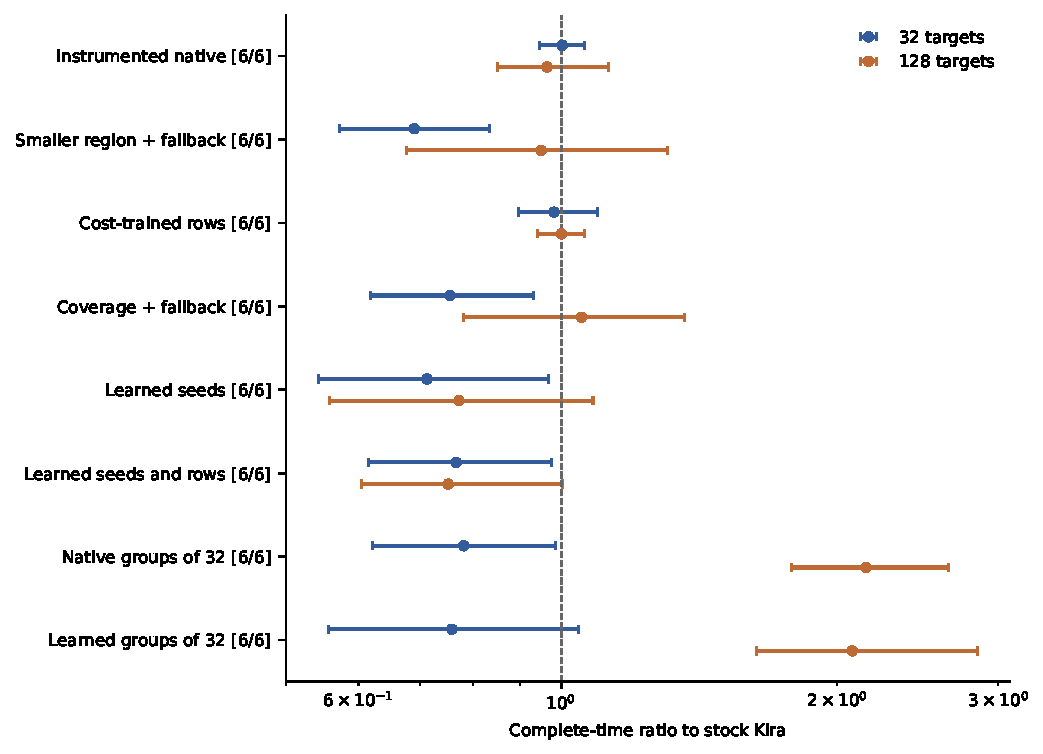
\includegraphics[width=\linewidth]{figures/native_multiloop_times.pdf}
\caption{Complete-time ratios to responsive stock Kira for 32 and 128 indexed targets. Points use medians of three exact repetitions and equal case weights. Bars show descriptive case-resampling intervals; the labels give complete paired batch counts. A ratio below one means lower measured time in the stated paired cohort.}
\label{fig:native-multiloop-times}
\end{figure}
\subsubsection{Repeated row decisions in the changing matrix}
The cost-trained row tree has a complete-time ratio of 1.008 with descriptive interval $[0.937,1.078]$ to the instrumented native policy. Its forward coefficient-operation ratio is 1.003 with descriptive interval $[0.983,1.021]$, while the measured forward-stage time ratio is 0.943 with descriptive interval $[0.828,1.033]$. The paired geometric mean forward times are 0.091 seconds for native choices and 0.085 seconds for the tree, while their complete times are 15.887 and 16.013 seconds. Most measured time therefore lies outside this recorded forward stage. The sampled continuation objective measures one altered source choice followed by native choices. Repeated tree choices change the later matrices and can therefore change the cost in a different direction. The full-workflow results determine whether the trained model saves work in this use.

The combined seed and row policy has a complete-time ratio of 0.759 with descriptive interval $[0.613,0.962]$ to responsive stock Kira. Its paired geometric mean median time is 12.280 seconds, compared with 11.998 seconds for seeds alone. The row addition therefore does not lower this point estimate. Combining two decisions requires a separate measurement because a different seed set changes the equations on which the row policy acts.

\begin{figure}[htbp]
\centering
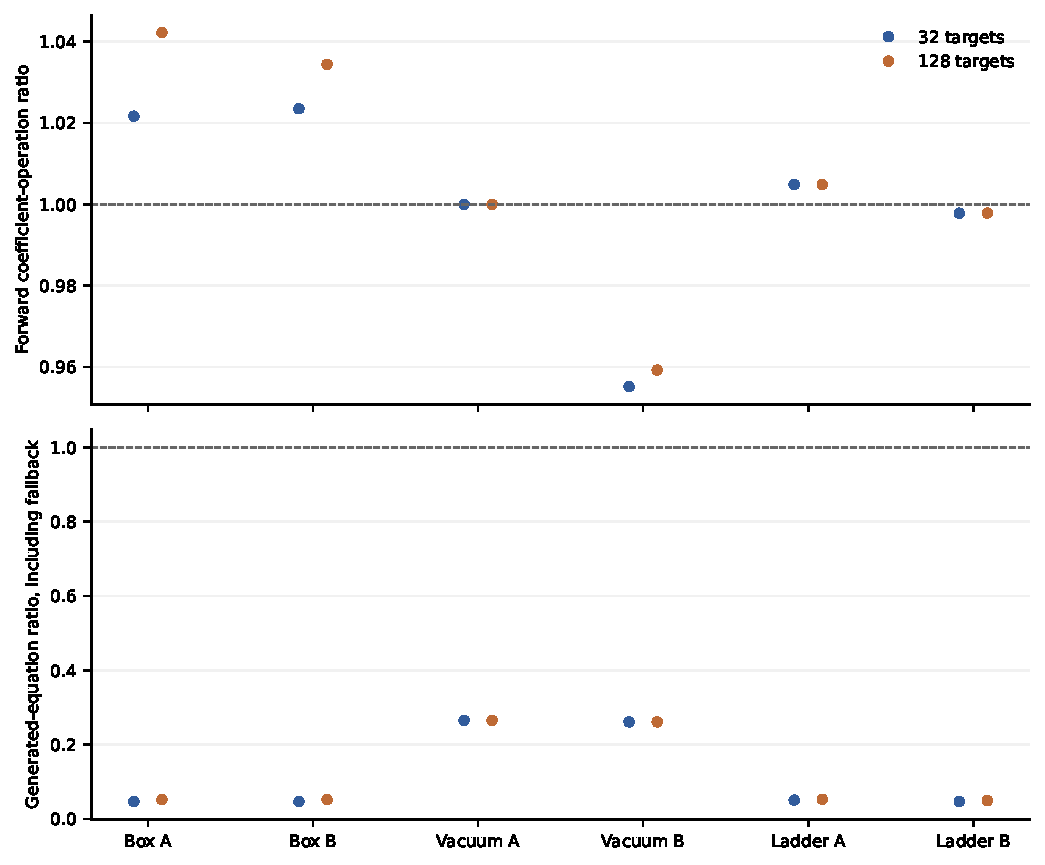
\includegraphics[width=\linewidth]{figures/native_multiloop_operations.pdf}
\caption{Per-case median work ratios in the reserved comparison. The row panel measures committed forward coefficient operations relative to the same instrumented native policy. The seed panel measures initial generated equations, summed over attempts, relative to native Kira. Cases A and B follow the parameter order given in the text. Counts concern different stages and do not measure Fermat's internal polynomial work.}
\label{fig:native-multiloop-operations}
\end{figure}
\subsubsection{Completion of larger target batches}
With 32 targets, responsive stock Kira completed 18 of 18 trials. For the learned seed workflow, 18 of 18 completed, including 6 rescued by fallback. For the combined workflow, 18 of 18 completed, including 6 rescued by fallback. For native groups of 32 targets, 18 of 18 completed, including 0 rescued by fallback. For combined groups of 32 targets, 18 of 18 completed, including 6 rescued by fallback. 

With 128 targets, responsive stock Kira completed 18 of 18 trials. For the learned seed workflow, 18 of 18 completed, including 6 rescued by fallback. For the combined workflow, 18 of 18 completed, including 6 rescued by fallback. For native groups of 32 targets, 18 of 18 completed, including 18 rescued by fallback. For combined groups of 32 targets, 18 of 18 completed, including 18 rescued by fallback. 

For 128 targets, splitting the native workflow gives a time ratio of 2.151 with descriptive interval $[1.783,2.647]$ to stock Kira. Splitting the combined workflow gives 2.078 with descriptive interval $[1.631,2.845]$. The separate fallback counts show whether completion improves; the paired times include repeated generation and process startup.

\begin{figure}[htbp]
\centering
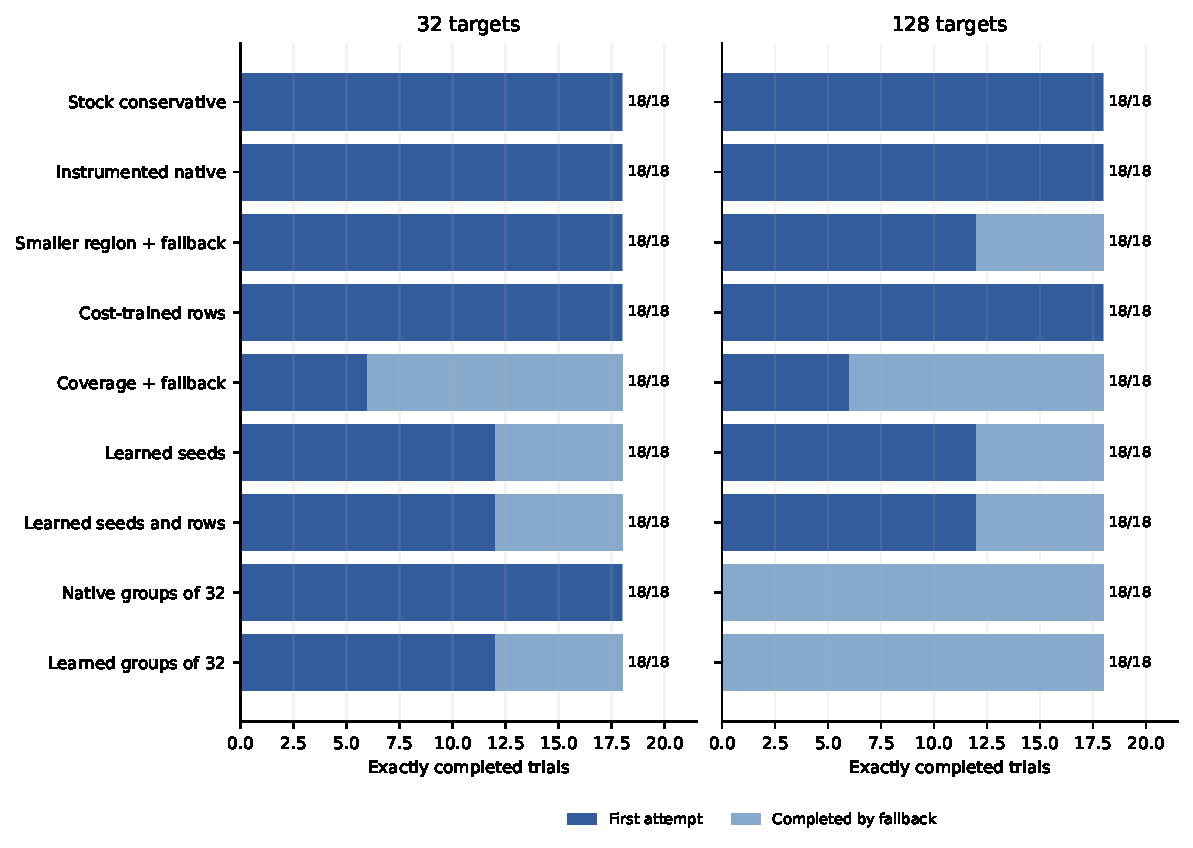
\includegraphics[width=\linewidth]{figures/native_multiloop_completion.pdf}
\caption{Completion of all requested targets under the fixed time and storage limits. The filled components distinguish successful initial reductions from reductions completed through fallback. Unfilled trials include failed or explicitly skipped outcomes. Each policy has eighteen planned trials at each batch size.}
\label{fig:native-multiloop-completion}
\end{figure}
\subsubsection{Scope and resource outcomes}
The largest recorded production process-tree memory use was 106.8 MiB, and the largest monitored production scratch allocation was 1.0 MiB. Among unsuccessful attempts, 7 logs report an allocation failure and 10 report recursive termination; these diagnostic counts can overlap. The fixed process limits constrain these outcomes, and the logs alone do not establish exhaustion of physical RAM. The workflow retains their costs and follows the same fallback rule. A separate post-comparison check repeated the smaller seed region for the 128-target validation box using both the responsive stock executable and the instrumented native executable. Both reported \texttt{std::bad\_alloc} under the same solver limits, so this failure also occurs without the row-policy hook. This check concerns the failure mechanism and supplies no additional timing comparison; it leaves all frozen reserved settings unchanged.

One scheduler interruption stopped a test worker when the sum of its processes' virtual address spaces exceeded the job limit. We preserved its completed records and resumed only missing work with a larger scheduler address-space allowance, while keeping the measured physical-memory, scratch and elapsed-time limits fixed. This interruption is recorded separately from completed workflow timings. With the resumed case excluded, the learned seed to stock complete-time ratio is 0.676 with descriptive interval $[0.549,0.963]$. With the resumed case excluded, the learned row to native complete-time ratio is 1.039 with descriptive interval $[0.991,1.102]$. The tests include two- and three-loop systems at fixed rational kinematics, a finite prescribed seed region and a restricted source-row action. They do not establish a speedup for arbitrary symbolic kinematics, every multiloop topology, or the earlier restricted collection through twelve loops.
\FloatBarrier
